%%
%% Odor Transformation Rules Paper
%% Using Elsevier CAS Single Column Template
%%

\documentclass[a4paper,fleqn]{cas-sc}

\usepackage[authoryear,longnamesfirst]{natbib}
\usepackage{amsmath}
\usepackage{amssymb}
\usepackage{booktabs}
\usepackage{multirow}
\usepackage{array}
\usepackage{subcaption}
\usepackage{float}

% Graphics path - all figures in local figures/ directory
\graphicspath{{figures/}}

\begin{document}
\let\WriteBookmarks\relax

% Short title for running header
\shorttitle{From Metabolic Operators to Perceptual Transitions}

% Short author for running header
\shortauthors{Author et~al.}

% Main title
\title[mode=title]{From Metabolic Operators to Perceptual Transitions: First-Order Rule Mining and Auditable Logical Reasoning for Mechanistic Olfaction}

% First author
\author[1]{First Author}
\cormark[1]
\ead{author@example.edu}
\credit{Conceptualization, Methodology, Software, Writing - Original Draft}

\affiliation[1]{organization={Department of Computer Science},
            addressline={University Name},
            city={City},
            postcode={000000},
            country={Country}}

% Corresponding author text
\cortext[1]{Corresponding author}

% Abstract
\begin{abstract}
Structure--odor models locate molecules in perceptual space but do not explain how perceptions change under biochemical transformations. We introduce a transformation-centric framework that treats enzyme sequences as transformation sequences over odor categories and mines first-order logic rules as testable constraints on these sequences. Using The Good Scents Company (TGSC) odor annotations and KEGG (Kyoto Encyclopedia of Genes and Genomes) main-pair reactions, we build an odor-centered metabolic graph and project pathway-derived Cartesian odor events $(S, \mathbf{E}, T)$. From these events we extract 11,560 interpretable rules and compile them into a Prolog-style (logic-programming) inference engine that supports deduction, abduction, and contradiction checking with explicit proof traces. The resulting rulebook highlights lyase-dominated transformations and identifies the terpene-cyclase class Enzyme Commission (EC)~4.2.3 as a recurrent mediator between citrus, fresh, herbal, and floral odors, generating falsifiable hypotheses for metabolic engineering and sensory studies. Crucially, the logic exposes directional and exclusionary sequence constraints---a non-commutative, boundary-defined odor logic that challenges purely structural views of olfaction. All rules, reasoning tools, and proof-trace demonstrations are publicly available.
\end{abstract}

% Research highlights
\begin{highlights}
\item A transformation-centric model treats enzyme sequences as transformation sequences that drive odor-to-odor transitions rather than static labels.
\item Cartesian odor events enable first-order rule mining and auditable reasoning with proof traces.
\item Lyase-dominated pathways and EC~4.2.3 emerge as recurrent mediators of citrus-to-fresh/floral transitions.
\item The rulebook yields falsifiable hypotheses relevant to metabolic engineering and sensory validation.
\end{highlights}

% Keywords
\begin{keywords}
olfactory perception \sep metabolic pathways \sep odor transformation \sep first-order logic \sep logical reasoning \sep proof trace \sep abductive inference \sep KEGG \sep enzyme sequences
\end{keywords}

\maketitle

%% ============================================================
\section{Introduction}\label{sec:intro}
%% ============================================================

% --- Paragraph 1: Neuroscience gap ---
Olfaction---the sense of smell---enables organisms to detect and discriminate thousands of volatile molecules, guiding behaviors from food selection to mate recognition \citep{Buck1991,Leffingwell2002}. The computational quest to decode this ability has long focused on the \emph{structure-odor relationship} (SOR): mapping molecular descriptors to perceptual labels \citep{Rossiter2012,Keller2017,Chacko2019}. Recent models embed molecules into perceptual spaces with graph neural networks and multitask predictors \citep{Lee2023,Song2025}. Yet these approaches share a blind spot: they explain \emph{where} a molecule lies in perceptual space, but not \emph{how} perceptual states move under biochemical transformations. Human olfactory experience unfolds through fermentation, ripening, cooking, and decay, processes in which one odor \emph{becomes} another \citep{Schwab2008,Dunkel2014}. A science of olfaction that cannot describe these transitions is incomplete, and a purely structural view misses a deeper question: what \emph{rules} govern which odor transitions are possible, impossible, or directionally constrained?

% --- Paragraph 2: Metabolism gap ---
The missing link is metabolism. Odorants are rarely isolated end-products; they are intermediates along enzymatic cascades that interconvert molecular structures \citep{Schwab2008}. Terpenes in citrus fruits arise through cyclization by terpene synthases; esters in fermented beverages are assembled by acyltransferases; aldehydes in aged foods accumulate via oxidoreductase-mediated degradation \citep{Tholl2015,Hazelwood2008,Dunkel2014}. Existing olfactory databases---The Good Scents Company (TGSC) \citep{TGSC2024}, Pyrfume \citep{Sharma2024}, and others---record each compound's odor as a static annotation, compressing the dynamic of biosynthetic and degradative routes into flat labels. By grounding odor relations in KEGG reaction main-pairs \citep{Kanehisa2021}, we can instead treat metabolism as a mechanistic generator of odor transitions rather than background annotation.

% --- Paragraph 3: Logic / explainable-AI gap ---
Even when transformations are recovered, converting them into \emph{scientific knowledge} demands more than statistical summaries. Many explainable artificial intelligence (AI) methods offer local, post-hoc rationales for individual predictions but cannot express the compositional constraints that govern odor transformations: ``\emph{must} pass through a lyase,'' ``\emph{cannot} reach a cheesy target,'' ``these two enzyme classes \emph{never co-occur}.'' First-order logic provides the expressive vocabulary for such constraints, and Prolog-style (logic-programming) backward chaining provides an inference mechanism that can derive new conclusions with explicit proof traces---turning descriptive patterns into \emph{executable, auditable hypotheses} \citep{Muggleton1994,Cropper2022}.

% --- Core claim ---
\medskip
\noindent\textbf{Core thesis.}
We propose a \emph{transformation-centric} mid-level framework in which enzyme sequences act as generative transformation sequences over perceptual odor categories, and first-order logic rules encode falsifiable constraints on these sequences. The goal is to model odor not as a static molecular property but as a queryable, mechanistically grounded, and logically auditable transformation process---bridging metabolic chemistry, sensory neuroscience, and symbolic reasoning within a single formal object: the \textbf{Cartesian odor event} $(S, \mathbf{E}, T)$. This framing makes a stronger claim than ``structure predicts odor'': it asserts that odor space is governed by a sequence grammar with directionality and boundaries, and that these constraints can be discovered and audited.

The next section summarizes the key results and cross-disciplinary contributions in a narrative form; related work, data and methods, and quantitative analyses follow in later sections.

\begin{figure}[pos=H]
	\centering
	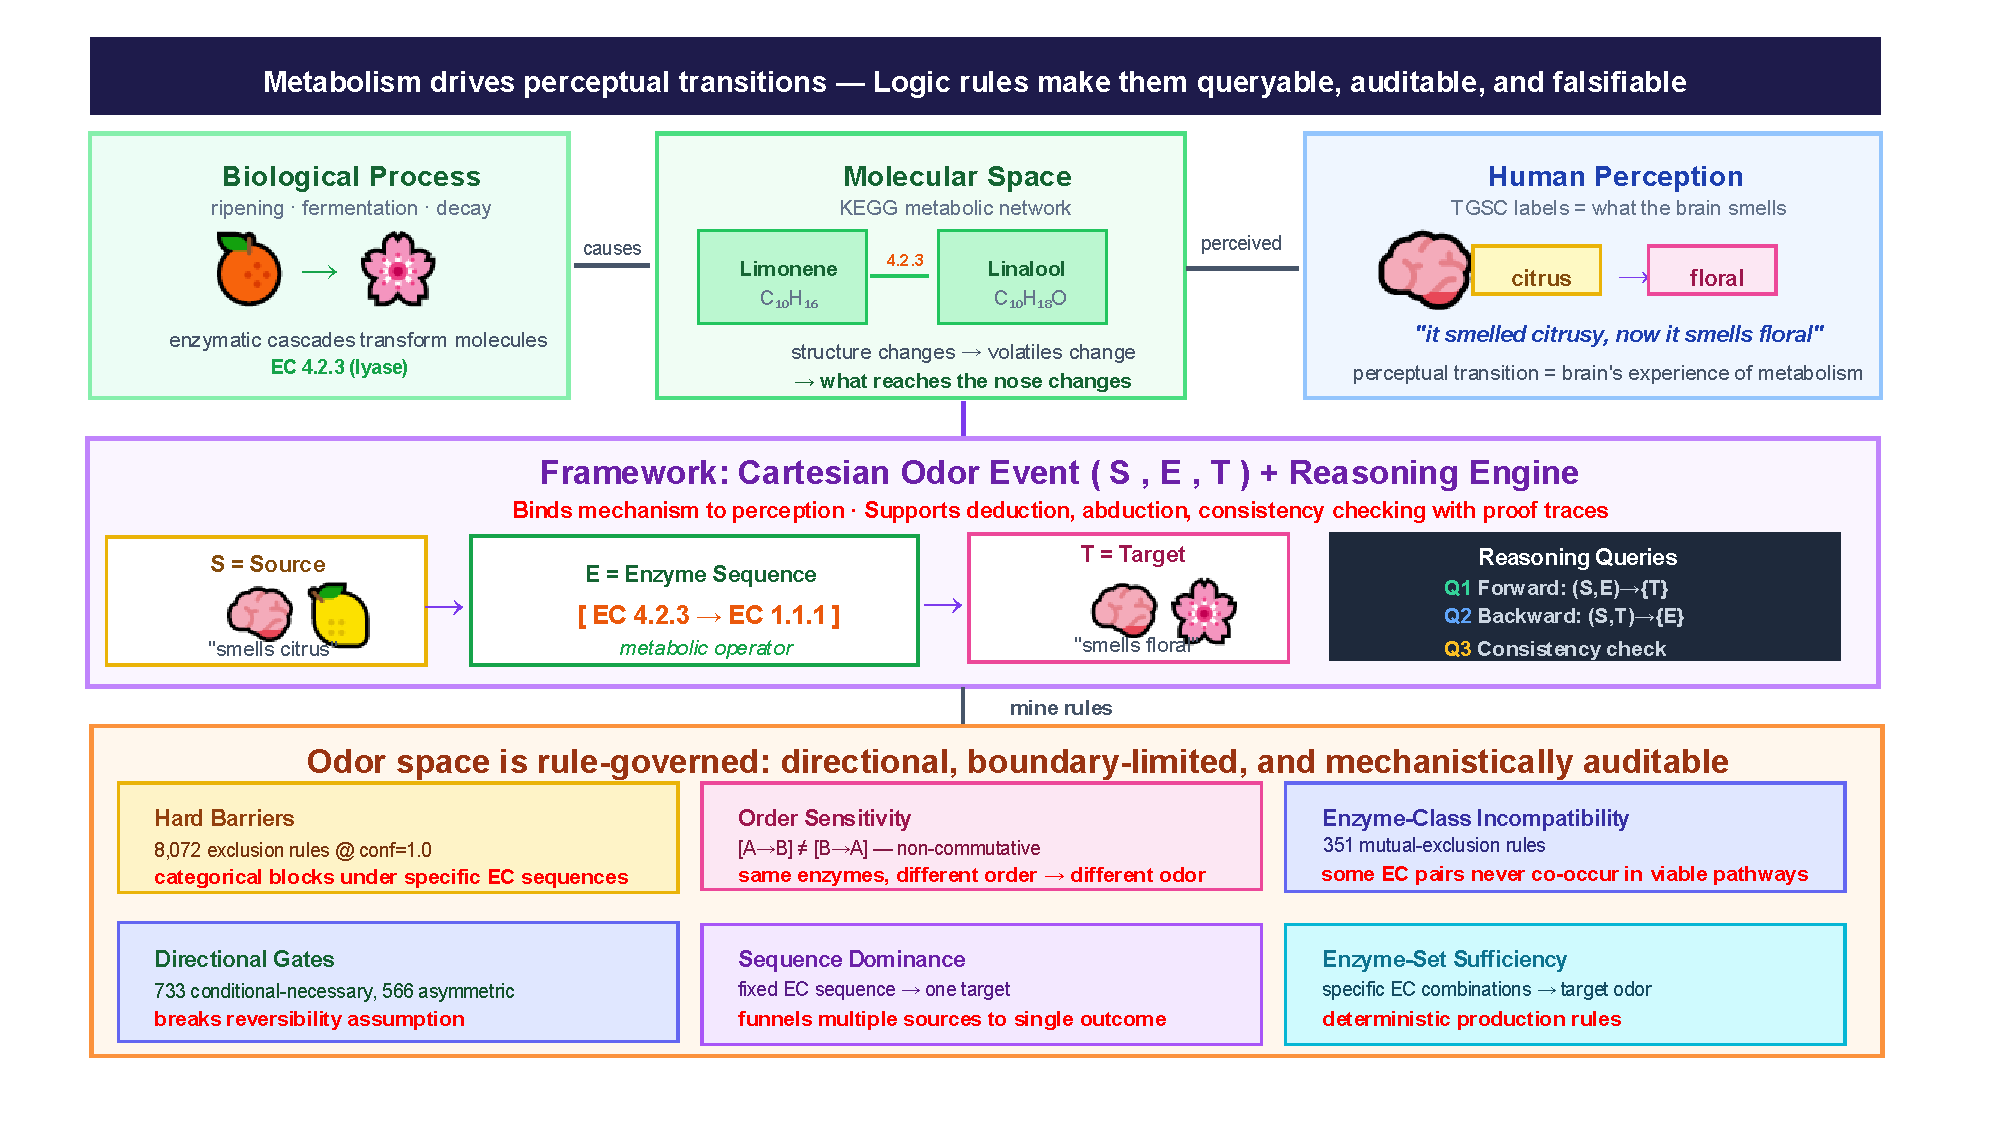
\includegraphics[width=\linewidth]{overview.pdf}
	\caption{Overview of the transformation-centric pipeline: data sources, Cartesian odor events, rule mining, and logic-based reasoning outputs.}
	\label{fig:overview}
\end{figure}

%% ============================================================
\section{Results and Cross-Disciplinary Contributions}\label{sec:key-results}
%% ============================================================

Figure~\ref{fig:overview} provides a compact overview of the workflow and outputs: odor annotations and KEGG reactions are lifted into Cartesian odor events, mined into first-order rules, and compiled into an auditable reasoning layer with queryable proof traces.



At a high level, this study delivers a mechanistic bridge between odor categories and biochemical transformations. By combining TGSC odor annotations with KEGG reaction knowledge and main-pair filtering, we convert scattered molecule--odor labels into a pathway-derived odor event space in which a statement such as ``citrus becomes floral via EC~4.2.3'' is a formal, queryable object rather than an anecdotal observation \citep{Sharma2024,Kanehisa2021,Tholl2015}. This representation makes the biology explicit while keeping the perceptual vocabulary that matters to olfaction researchers and flavor scientists \citep{Schwab2008,Dunkel2014}.

The rulebook reveals interpretable enzymatic motifs that align with known biochemical routes. A recurrent pattern is the prominence of lyases, particularly EC~4.2.3 terpene cyclases, which repeatedly mediate transitions among citrus, fresh, herbal, and floral categories; this mirrors the central role of terpene cyclization in monoterpenoid biosynthesis \citep{Tholl2015,Kanehisa2021}. Another example is a fruity$\rightarrow$fishy transition associated with aminotransferase and decarboxylase sequences, consistent with Ehrlich-pathway chemistry in fermentation contexts \citep{Hazelwood2008}. These are not merely frequency counts: they are method-derived, pathway-grounded hypotheses that tie perceptual shifts to enzyme logic documented in biochemical literature \citep{Schwab2008,Dunkel2014}.

More importantly, the rules reveal a set of \emph{distinct} and disruptive properties of odor transformation that are difficult to see in purely structure-based models. The key point is that these are \emph{logical constraints}---not just correlations---because each property is encoded as a first-order rule that can be queried, chained, and contradicted. \textbf{Hard barriers} appear as \emph{exclusion rules} (e.g., \texttt{from(citrus) and via([4.2.3 -> 4.2.3]) -> not to(cheesy)}), showing categorical blocks under specific enzyme sequences; this resonates with thermodynamic irreversibility constraints that forbid certain reaction directions in metabolic networks \citep{Kummel2006,Martinez2014}. \textbf{Enzyme-class incompatibility} appears as \emph{mutual-exclusion rules} (e.g., \texttt{via\_ec(P, 6.2.1) and via\_ec(P, 4.2.3) -> false}), indicating that some enzyme classes cannot co-occur in a valid chain and echoing flux-coupling notions of incompatible reaction pairs \citep{Hosseini2017}. \textbf{Directional gates} appear as \emph{conditional-necessary rules} (e.g., \texttt{from(citrus) and to(floral) -> must\_via(4.2.3)}), breaking reversibility and aligning with thermodynamics-based directionality assignments \citep{Haraldsdottir2012}. \textbf{Sequence dominance} appears as \emph{disjunctive-source rules} where a fixed sequence funnels multiple sources to one target, consistent with enzyme-controlled product distributions in terpene biosynthesis \citep{Raz2020}. \textbf{Enzyme-set sufficiency} appears as \emph{sufficient rules} (e.g., \texttt{via\_ec(P, 2.5.1) and via\_ec(P, 2.6.3) and via\_ec(P, 4.1.3) and via\_ec(P, 4.1.99) -> produces(P, floral)}), paralleling evidence that terpene synthases can largely dictate product specificity \citep{Raz2020,Rudolf2020}. \textbf{Order sensitivity} appears in \emph{chain rules} where swapping the order of the same steps changes the implied transition, highlighting sequence-level semantics rather than set membership; this echoes assembly-line biosynthesis where module order determines product structure \citep{Nava2023,Nivina2019}.

These are not rhetorical claims; they are supported by rule counts and examples, and the logic makes them checkable. We find 8,072 exclusion rules at confidence 1.0 (\textbf{hard barriers}), 351 mutual-exclusion rules with confidence $\geq$ 0.9 (\textbf{enzyme-class incompatibility}), and 733 conditional-necessary source$\rightarrow$target pairs with 566 asymmetric (\textbf{directional gates}). \textbf{Sequence dominance} and \textbf{enzyme-set sufficiency} appear in disjunctive-source and sufficient rules with confidence 1.0 (support 54 and 11, respectively). \textbf{Order sensitivity} is visible even in two-step chain rules, where reversing the order of the same pair yields sulfurous$\rightarrow$mint/cooling/camphoreous in one direction and phenolic$\rightarrow$burnt/sulfurous in the other. Figure~\ref{fig:boundary_rules} summarizes these signals and illustrates the order effect.

\begin{figure}[pos=H]
    \centering
    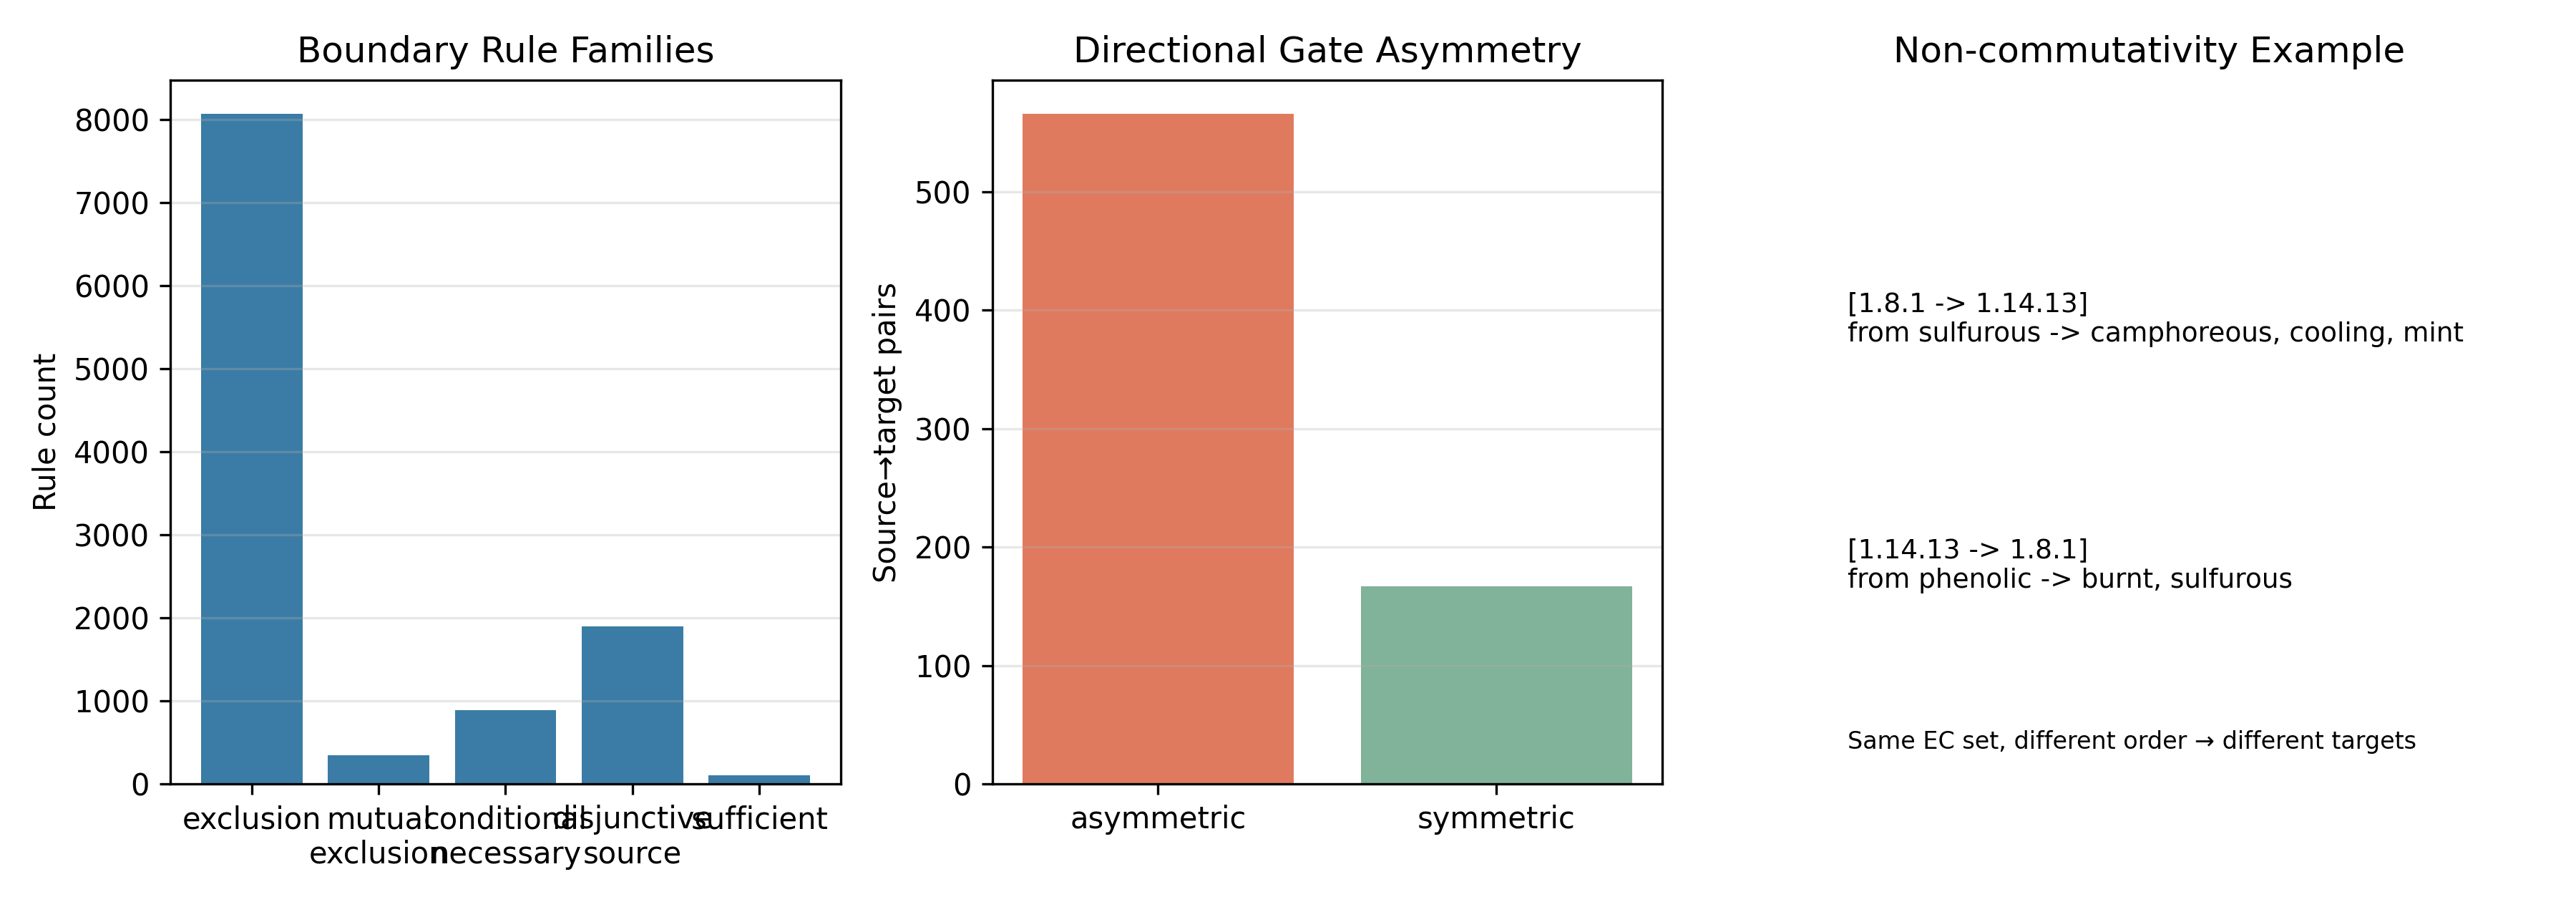
\includegraphics[width=\linewidth]{10_rule_boundaries.png}
    \caption{Boundary and directionality evidence from KEGG-only rules. (A) Counts of boundary-related rule families. (B) Asymmetry in conditional-necessary source$\rightarrow$target pairs. (C) Non-commutativity example: the same EC set in different order yields different odor transitions (chain rules are extracted with a permissive threshold to reveal sequence effects).}
    \label{fig:boundary_rules}
\end{figure}

The most disruptive insight is that the rulebook defines a \emph{directional} and \emph{boundary-limited} odor logic. We observe enzyme sequences whose \emph{order} changes the implied odor transition (swapping two EC steps yields different source$\rightarrow$target patterns), a non-commutative behavior that cannot be captured by static embeddings of molecular structure. We also recover strong exclusion and mutual-exclusion constraints that carve out ``impossible'' regions of odor space, indicating that certain odor targets are mechanistically inaccessible under specific enzyme steps or step pairs. Together these findings imply that odor space is not just a geometric map but a rule-governed process with explicit prohibitions and directionality, opening a new class of falsifiable claims for experimental testing.

Equally important is the cross-disciplinary value of the reasoning layer. First-order rules compiled into a Prolog-style engine support deduction, abduction, and contradiction checking with proof traces, aligning with long-standing insights from logic programming and inductive logic learning \citep{Muggleton1994,Cropper2022}. Those proof traces translate computational patterns into falsifiable, experiment-ready hypotheses, which is precisely the kind of structure sought in metabolic engineering and sensory validation workflows \citep{MetabolicEngineering2024,Dunkel2014}. The result is not a replacement for structure--odor modeling but a complementary lens: while SOR models locate molecules in perceptual space, the rulebook constrains \emph{how} that space can be traversed by biochemical transformation steps \citep{Rossiter2012,Keller2017,Lee2023,Song2025}. Taken together, the central value proposition is a mechanistically grounded, auditable rule system that makes cross-disciplinary claims testable rather than merely descriptive.

%% ============================================================
\section{Related Work}\label{sec:related}
%% ============================================================

\subsection{Structure-odor relationship modeling}

The quest to predict odor from molecular structure has a long history. Early approaches relied on hand-crafted molecular descriptors correlated with perceptual categories. \citet{Keller2017} demonstrated that random forest models could predict odor pleasantness and intensity from physicochemical features. Recent advances employ deep learning: \citet{Lee2023} used graph neural networks to generate a continuous Principal Odor Map (POM) that preserves perceptual similarities. \citet{Song2025} developed multitask models capturing shared representations across related odor categories. \citet{Chacko2019} applied subgroup discovery algorithms to identify physicochemical rules discriminating odor qualities.

However, \emph{none of these approaches model odor as a transformation}. They treat each molecule as an isolated data point, ignoring metabolic pathways connecting odorants.

\subsection{Odor datasets and resources}

Several databases provide molecule-odor annotations. \citet{Sharma2024} unified over 40 olfactory datasets into the Pyrfume framework, comprising $>$20,000 unique odorants. The Good Scents Company (TGSC) provides detailed odor descriptors for $>$4,000 compounds \citep{TGSC2024}. These datasets provide \emph{static} molecule-odor mappings; our contribution is to \emph{connect} these annotations through metabolic pathways.

\subsection{Metabolic pathway databases}

KEGG (Kyoto Encyclopedia of Genes and Genomes) provides a comprehensive resource linking compounds, reactions, enzymes, and pathways \citep{Kanehisa2021}. KEGG's reaction-class (RCLASS) database defines reaction patterns at the chemical bond level, with ``main-pairs'' specifying dominant substrate-product relationships. We leverage main-pairs to ensure biochemically meaningful pathways.

\subsection{Terpene biosynthesis and flavor chemistry}

Terpenes exemplify the metabolic origin of odorants. The methylerythritol phosphate (MEP) and mevalonate (MVA) pathways produce isoprene precursors, which terpene synthases convert to monoterpenes and sesquiterpenes \citep{Tholl2015}. The Ehrlich pathway generates fusel alcohols during fermentation \citep{Hazelwood2008}. Our framework captures these transformations through lyase-dominated EC sequences.

\subsection{Logic programming and explainable AI in the sciences}

Logic programming languages---Prolog and its descendants---have a long history in bioinformatics for representing metabolic rules, gene regulatory constraints, and pharmacological knowledge \citep{Muggleton1994}. Inductive Logic Programming (ILP) learns first-order rules from relational data, offering human-readable hypotheses with formal proof semantics \citep{Cropper2022}. In the explainable-AI landscape, most methods (SHapley Additive exPlanations, SHAP; Local Interpretable Model-agnostic Explanations, LIME; attention maps) provide post-hoc, instance-level rationales; in contrast, first-order rules are \emph{global, compositional, and executable}: they can be chained into multi-step proofs, checked for consistency, and used to derive novel conclusions---capabilities absent from feature-attribution approaches. To our knowledge, no prior work has applied Prolog-style deductive reasoning with proof traces to olfactory perception or odor transformation data.

%% ============================================================
\section{Materials and Methods}\label{sec:methods}
%% ============================================================

\subsection{Data sources}

\subsubsection{TGSC odor annotations}
We obtained odor descriptor annotations from The Good Scents Company \citep{TGSC2024}, mapped to KEGG compound identifiers. After filtering for valid KEGG IDs and excluding odorless compounds, 542 odorous compounds formed the seed set spanning 138 binary odor attributes.

\subsubsection{KEGG reaction network}
Reaction-compound links were downloaded from the KEGG REST (Representational State Transfer) API. Each reaction is annotated with EC (Enzyme Commission) numbers, the standard classification of enzyme families by reaction type. Ubiquitous carrier molecules (water, adenosine triphosphate (ATP), nicotinamide adenine dinucleotide (NAD$^+$), coenzyme A (CoA), etc.---37 compounds total) were blacklisted to prevent spurious connectivity.

\subsubsection{Main-pair filtering}
To ensure biochemically meaningful substrate-product relationships, we applied KEGG's RCLASS main-pair data, achieving 76.6\% coverage of reactions.

\subsection{Odor-centered network construction}

Starting from 542 odorous compounds, we expanded the network to depth 2 in the KEGG reaction graph. The resulting network contains 4,186 nodes (542 odorous compounds, 1,747 intermediates, 1,897 reactions), 7,237 directed edges, and 1,769 reactions with EC annotations.

\subsection{Pathway enumeration}

For each pair of odorous compounds, we enumerated reaction paths up to length 5 using breadth-first search, retaining at most 2 paths per compound pair. This yielded 25,554 pathways.

\subsection{Cartesian odor event projection}

Each pathway was projected into odor space. If compound $A$ with odor labels $\{s_1, s_2, \ldots\}$ transforms via enzyme sequence $\mathbf{E}$ to compound $B$ with odor labels $\{t_1, t_2, \ldots\}$, we generate all combinations $(s_i, \mathbf{E}, t_j)$. This Cartesian expansion produced 178,450 total odor events, 129,738 unique triplets, and 10,286 unique EC sequences.

\subsection{First-order logic rule mining}

We extracted six classes of first-order logic rules, each expressed as a Horn-style template that supports downstream reasoning:
\begin{align*}
\textbf{Necessary:}\quad & \forall P: \texttt{transforms}(S, T, P) \rightarrow \texttt{via\_ec}(P, E) \\
\textbf{Sufficient:}\quad & \bigwedge_i \texttt{via\_ec}(P, E_i) \rightarrow \texttt{produces}(P, T) \\
\textbf{Exclusion:}\quad & \texttt{from}(S) \wedge \texttt{via}(E) \rightarrow \neg\texttt{to}(T) \\
\textbf{Disjunctive source:}\quad & (\texttt{from}(S_1) \vee \texttt{from}(S_2)) \wedge \texttt{via}(E) \rightarrow \texttt{to}(T) \\
\textbf{Mutual exclusion:}\quad & \texttt{via}(E_1) \wedge \texttt{via}(E_2) \rightarrow \bot \\
\textbf{Conditional necessary:}\quad & \texttt{from}(S) \wedge \texttt{to}(T) \rightarrow \texttt{must\_via}(E)
\end{align*}

Rules were filtered by minimum support (2.0) and confidence thresholds (0.8--0.95 depending on rule type).

\subsection{Queries over odor transformations}\label{sec:queries}

The six rule types define a space of structured queries over odor transformations. We formalize three canonical query families that turn the extracted rules from a descriptive catalogue into an \emph{actionable reasoning system}:

\medskip
\noindent\textbf{Q1: Forward reasoning (deduction).}
Given a source odor $S$ and an enzyme constraint set $\mathbf{E}$, infer the set of plausible target odors:
\begin{equation}\label{eq:q1}
    (S, \;\mathbf{E}) \;\Rightarrow\; \{T \mid \text{consistent with all applicable rules}\}.
\end{equation}
Forward reasoning applies \emph{sufficient} rules (predicting targets) and \emph{exclusion} rules (eliminating impossible targets). The result is a ranked list of reachable odor categories together with a ``why-not'' set of excluded targets and the rules that block them.

\medskip
\noindent\textbf{Q2: Backward reasoning (abduction).}
Given a desired target odor $T$ (and optionally a source $S$), infer the enzymatic steps (EC classes) that are required or forbidden:
\begin{equation}\label{eq:q2}
    (S, \;T) \;\Rightarrow\; \{\mathbf{E}_{\text{required}}, \;\mathbf{E}_{\text{forbidden}}\}.
\end{equation}
Abductive queries leverage \emph{necessary} and \emph{conditional necessary} rules (identifying must-have enzymes) and \emph{exclusion} rules (identifying forbidden enzymes). This supports ``recipe-inverse'' applications: given a target fragrance profile, what enzymatic pathway constraints apply?

\medskip
\noindent\textbf{Q3: Consistency checking (contradiction detection).}
Given a candidate enzyme set $\mathbf{E}_{\text{cand}}$, determine whether the set is internally consistent:
\begin{equation}\label{eq:q3}
    \mathbf{E}_{\text{cand}} \;\Rightarrow\; \bot \quad\text{(contradiction)}\quad \text{or} \quad \checkmark \quad\text{(consistent)}.
\end{equation}
Consistency queries apply \emph{mutual exclusion} rules to detect enzyme pairs that never co-occur in viable pathways. When a contradiction is found, the proof trace identifies the conflicting rules, enabling pathway designers to pinpoint which constraint is violated.

\medskip
Table~\ref{tbl:querymap} maps each rule type to its primary reasoning function.

\begin{table}[pos=H]
\caption{Mapping from rule type to reasoning function}\label{tbl:querymap}
\begin{tabular*}{\tblwidth}{@{}LLL@{}}
\toprule
Rule Type & Reasoning Function & Query \\
\midrule
Necessary & Explanation (``why this enzyme?'') & Q2 \\
Sufficient & Generative prediction & Q1 \\
Exclusion & Negation (``why NOT this target?'') & Q1, Q2 \\
Disjunctive Source & Alternative pathway reasoning & Q1 \\
Mutual Exclusion & Conflict detection & Q3 \\
Conditional Necessary & Causal explanation & Q2 \\
\bottomrule
\end{tabular*}
\end{table}

\subsection{Prolog-style inference engine with proof traces}\label{sec:prolog}

To operationalize the queries defined above, we compile the extracted first-order rules into a Prolog-style backward-chaining inference engine. The compilation proceeds as follows:

\subsubsection{Rule compilation}
Each rule is translated into a Horn clause. For example, a necessary rule ``transforming fruity to anisic requires EC~2.1.1'' becomes:
\begin{verbatim}
required_ec(fruity, anisic, '2.1.1').
\end{verbatim}
An exclusion rule ``from citrus via [4.2.3] cannot reach cheesy'' becomes:
\begin{verbatim}
excluded(citrus, '4.2.3', cheesy).
\end{verbatim}
Derived rules support multi-step inference. For instance:
\begin{verbatim}
can_transform(S, T) :-
    required_ec(S, T, _),
    \+ excluded(S, _, T).
\end{verbatim}

\subsubsection{Backward chaining with unification}
The engine resolves queries by recursively matching goals against the knowledge base, applying Robinson's unification algorithm for variable binding. Variables in query templates (e.g., \texttt{?T} in \texttt{can\_transform(citrus, ?T)}) are systematically bound to constants that satisfy all applicable rules.

\subsubsection{Proof trace generation}
Every derivation produces an explicit \emph{proof trace}: an ordered sequence of $\langle$\textit{goal, matched-rule, bindings}$\rangle$ triples that records each inference step. Proof traces serve three purposes: they make predictions falsifiable by exposing explicit enzymatic premises; they support scientific debugging by showing which rule types dominate a conclusion; and they improve trust and auditability by explaining \emph{why} a target odor is predicted or excluded rather than providing an opaque score.

This three-layer capability hierarchy---\emph{retrieval} (matching rules), \emph{inference} (chaining rules to derive conclusions), and \emph{explanation} (visualizing proof traces)---distinguishes the system from static rule tables and from black-box models that lack compositional reasoning.

%% ============================================================
\section{Empirical Analyses}\label{sec:empirical}
%% ============================================================

\noindent\textbf{Empirical overview.}

We first summarize the scale of the transformation dataset and the structure it induces. Table~\ref{tbl:scale} shows the expansion from 25,554 metabolic pathways to 178,450 odor events (a 6.98$\times$ expansion), reflecting the combinatorial richness of multi-odor compounds and the large number of distinct EC-level sequences. This breadth matters because the rulebook is inferred from a wide transformation space rather than a narrow, cherry-picked subset.

\begin{table}[pos=H]
\caption{Summary statistics of the odor transformation dataset}\label{tbl:scale}
\begin{tabular*}{\tblwidth}{@{}LL@{}}
\toprule
Metric & Value \\
\midrule
Odorous compounds & 542 \\
Odor attributes & 138 \\
Network nodes & 4,186 \\
Network edges & 7,237 \\
Enumerated pathways & 25,554 \\
Odor transformation events & 178,450 \\
Unique triplets & 129,738 \\
Unique EC sequences & 10,286 \\
Total extracted rules & 11,560 \\
\bottomrule
\end{tabular*}
\end{table}

The distribution of odor sources and targets is asymmetric: fruity and balsamic dominate as sources, while floral and fruity lead as targets. Pathway lengths are predominantly multi-step, and source--target transitions concentrate in stable corridors such as citrus$\rightarrow$citrus and fruity-mediated hubs. At EC level-3, the dominant motifs are lyase-heavy (notably \texttt{4.2.3 -> 4.2.3}), and enzyme-sequence usage is non-uniform across source/target odor groups.

\begin{figure}[pos=H]
\centering
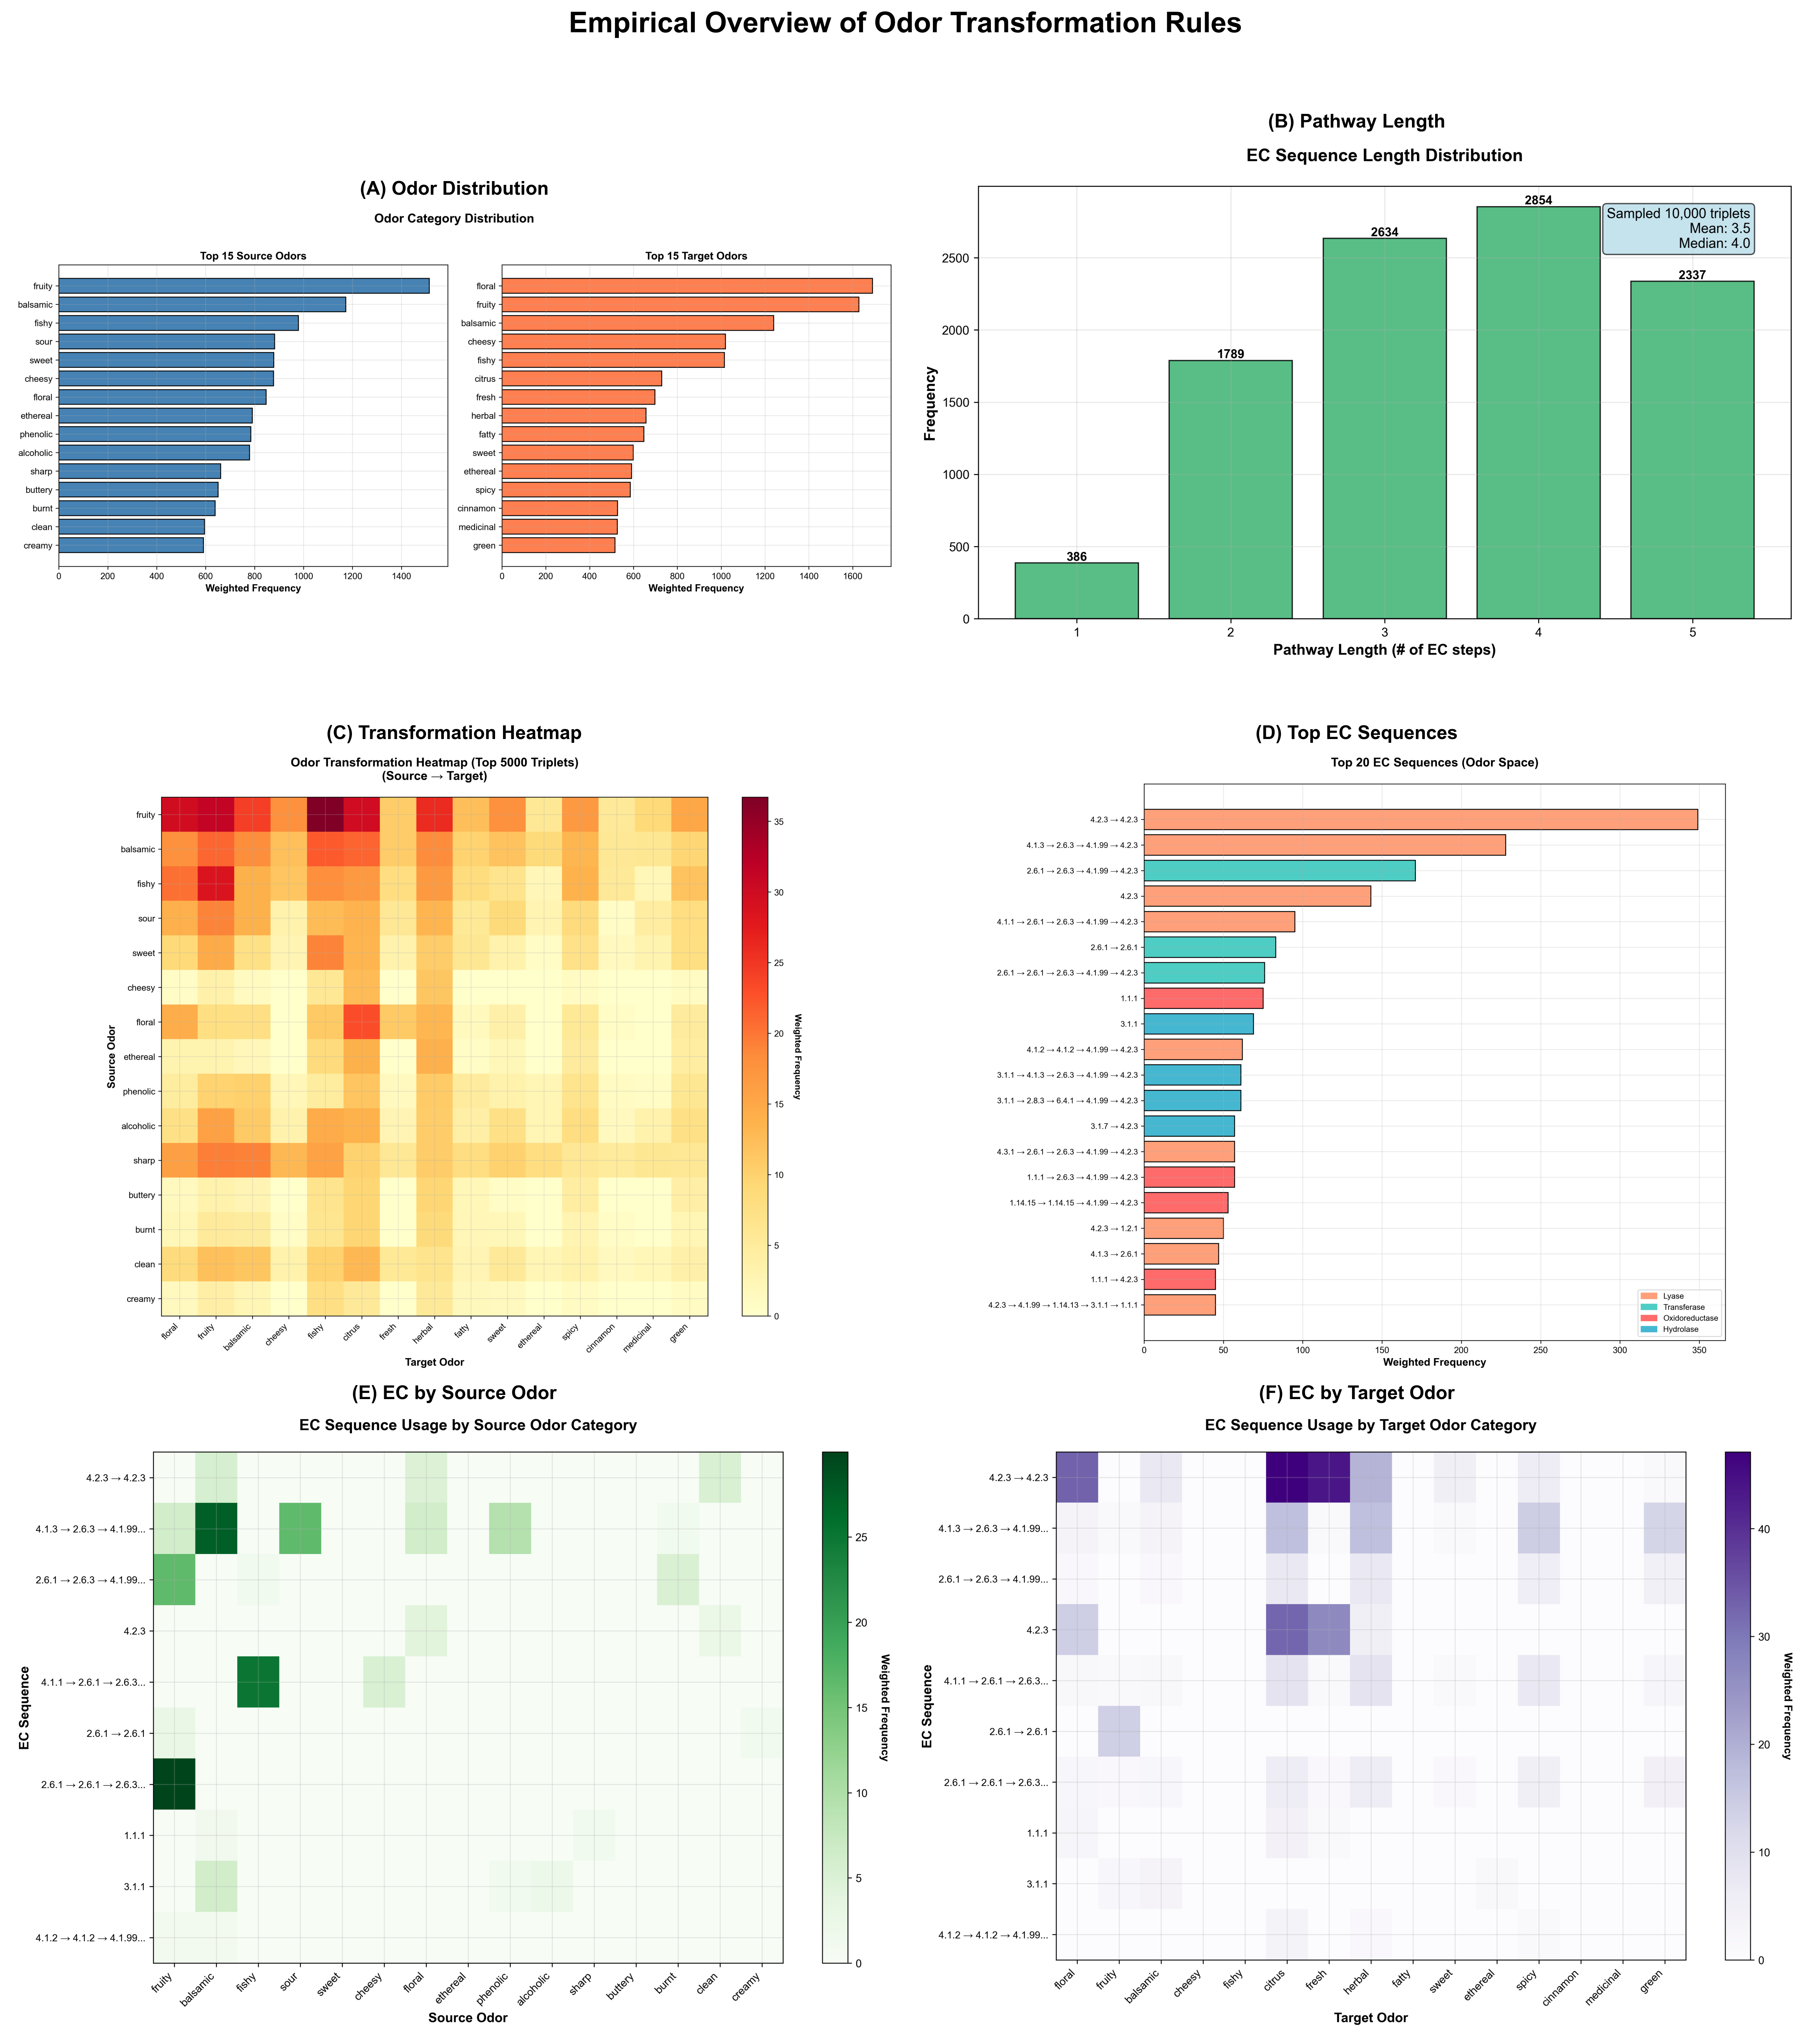
\includegraphics[width=\linewidth]{11_empirical_dashboard.png}
\caption{Composite empirical dashboard from V5 visualizations. (A) Source/target odor distribution. (B) Pathway length distribution. (C) Odor transformation heatmap. (D) Top EC sequences. (E) EC usage by source odor. (F) EC usage by target odor.}
\label{fig:empirical_dashboard}
\end{figure}

Figure~\ref{fig:empirical_dashboard} provides a compact empirical view of the transition space and its enzymatic organization, replacing multiple standalone plots with a single interpretable panel set.

\noindent\textbf{Enzymatic sequence statistics (EC level-3).}

At the functional-class level, lyases (EC 4.x) account for 47.9\% of pathway steps (Figure~\ref{fig:ecpie}), a striking departure from primary metabolism where oxidoreductases typically dominate. This supports the view that odor-relevant pathways are enriched for bond-cleaving, cyclization, and elimination chemistry that generates volatile structural diversity.

\begin{figure}[pos=H]
\centering
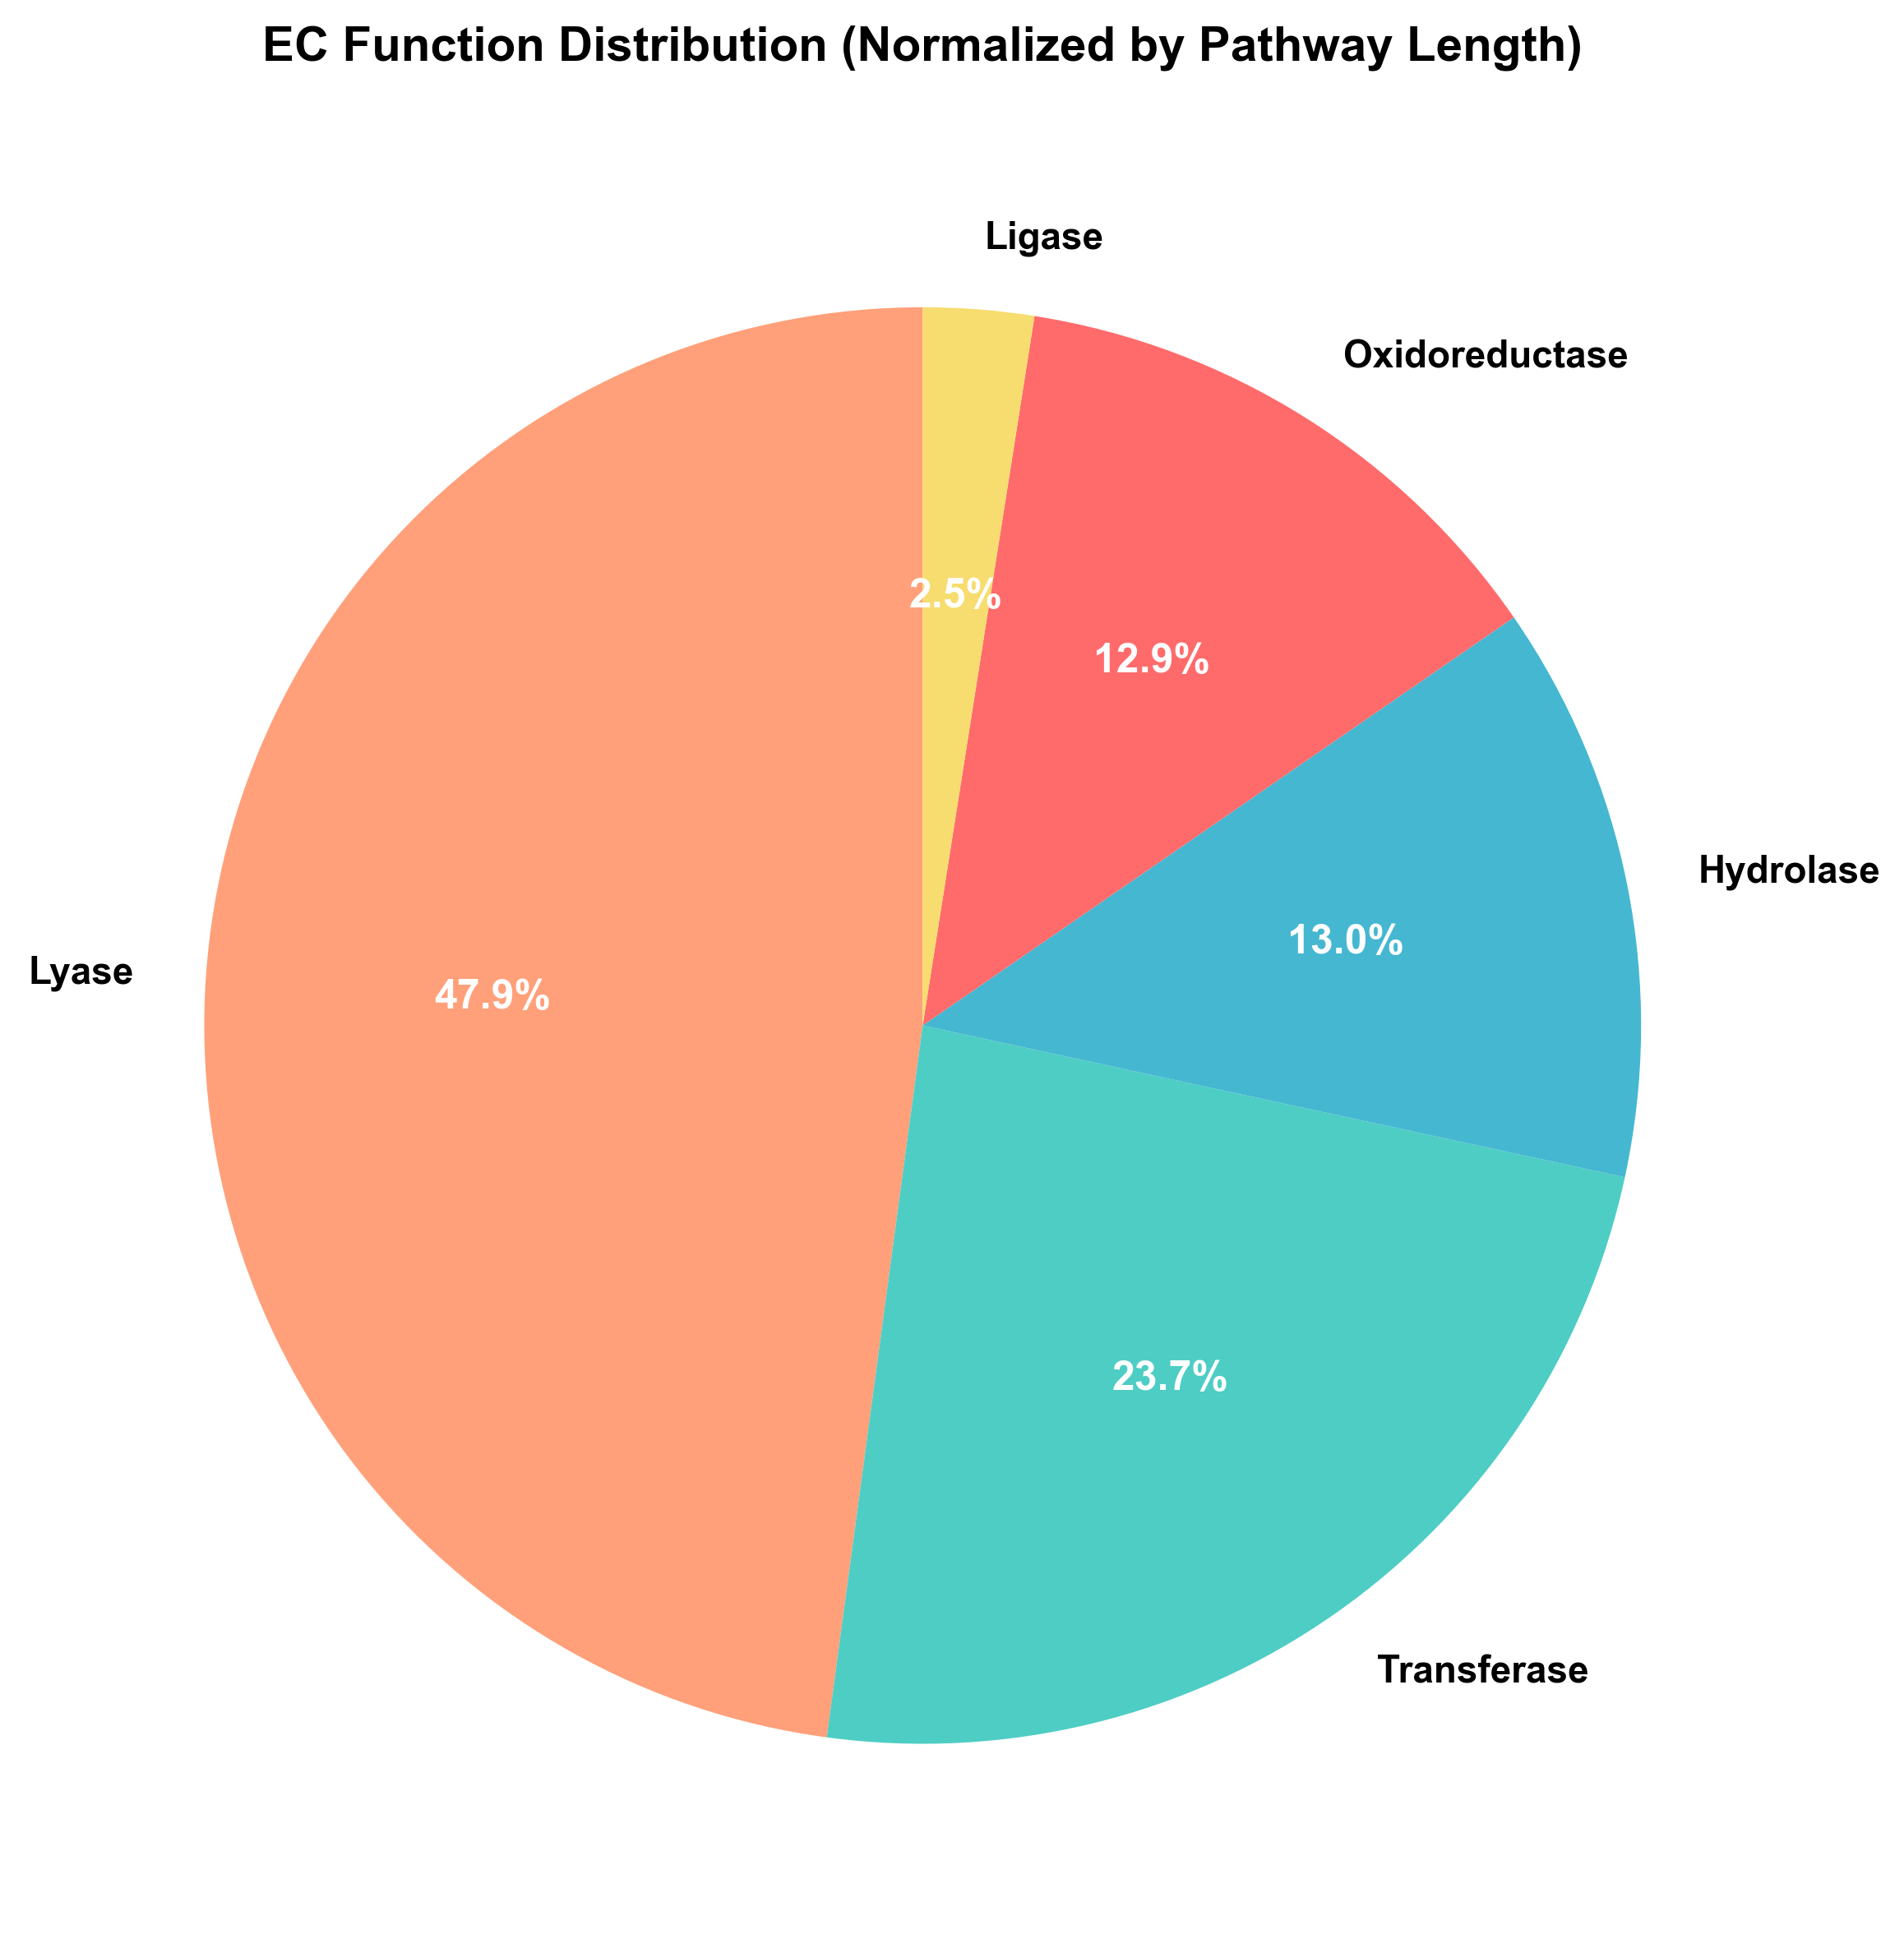
\includegraphics[width=0.6\linewidth]{08a_ec_function_pie_normalized.png}
\caption{Enzyme functional class distribution. Lyases dominate at 47.9\%.}
\label{fig:ecpie}
\end{figure}

\noindent\textbf{Rule mining and pathway alignment.}

Rules are mined as first-order constraints over EC-level sequences and odor transitions. Table~\ref{tbl:rules} summarizes the six rule families; the emphasis is not raw counts but the type of logical claim each family supports. Exclusion and mutual-exclusion encode negative constraints (what cannot happen), conditional-necessary encodes directional requirements (what must happen), while necessary and sufficient rules encode minimal or sufficient enzymatic evidence for a target.

This section anchors validation around two complementary checks. The first is biochemical: high-confidence rules should align with curated KEGG pathway logic (reported below). The second is perceptual and cross-dataset: rule-consistent transitions should be coherent with independent odor spaces such as the Principal Odor Map (POM) triplets \citep{Lee2023}. We outline this dual-anchor logic here to make the evaluation criteria explicit even before the cross-dataset analysis is presented in full.

\begin{table}[pos=H]
\caption{First-order logic rules extracted from odor transformation data}\label{tbl:rules}
\begin{tabular*}{\tblwidth}{@{}LLL@{}}
\toprule
Rule Type & Count & Example \\
\midrule
Exclusion & 8,072 & from(citrus) $\wedge$ via([4.2.3]) $\rightarrow$ $\neg$to(cheesy) \\
Disjunctive Source & 1,899 & (from(citrus) $\vee$ ...) $\wedge$ via(E) $\rightarrow$ to(T) \\
Conditional Necessary & 887 & from(citrus) $\wedge$ to(citrus) $\rightarrow$ must\_via(4.2.3) \\
Mutual Exclusion & 351 & via(6.2.1) $\wedge$ via(4.2.3) $\rightarrow$ $\bot$ \\
Necessary & 247 & transforms(fruity, anisic) $\rightarrow$ via(2.1.1) \\
Sufficient & 104 & via(4.1.3) $\wedge$ via(4.2.1) $\rightarrow$ produces(sweet) \\
\midrule
\textbf{Total} & \textbf{11,560} & \\
\bottomrule
\end{tabular*}
\end{table}

\noindent\textbf{Pathway-level validation against KEGG.}\label{sec:kegg-validation}

To test whether high-confidence rules recover known biochemistry, we traced the KEGG compound IDs behind the most frequent rule patterns and aligned them to pathway maps. Multiple rule-derived enzyme sequences correspond directly to well-characterized biosynthetic and catabolic routes, indicating that the rules capture established pathway logic without any pathway prior knowledge.

 \noindent\textbf{Confirmed pathway matches.}

\noindent\textbf{Monoterpenoid biosynthesis (KEGG map00902).} The highest-frequency rule, \emph{citrus} $\rightarrow$ \emph{citrus} via \texttt{[4.2.3]}, connects geranial (C01499) to multiple monoterpene products such as fenchol (C02344), terpinolene (C06075), and camphene (C06076). This aligns with monoterpenoid biosynthesis, where EC~4.2.3 terpene synthases/cyclases produce diverse cyclic terpenes from prenyl precursors. Specific KEGG branches within this EC class include EC~4.2.3.20 (geranyl diphosphate, GPP, $\rightarrow$ (R)-limonene), EC~4.2.3.25 (GPP $\rightarrow$ linalool), and EC~4.2.3.15 (GPP $\rightarrow$ myrcene), consistent with our observed citrus$\rightarrow$floral/fresh transitions. \citep{Kanehisa2021,Tholl2015}

\noindent\textbf{Ehrlich pathway / amino acid catabolism.} The rule \emph{fruity} $\rightarrow$ \emph{fishy} via \texttt{[2.6.1, 4.1.1]} maps to the Ehrlich pathway, where aminotransferases (EC~2.6.1) convert amino-acid-derived keto-acids and decarboxylases (EC~4.1.1) generate biogenic amines. The resulting amines are classic sources of fishy off-notes in fermentation and spoilage contexts, matching the perceptual transition captured by the rule. \citep{Hazelwood2008}

\noindent\textbf{Sulfur amino acid $\rightarrow$ alcohol (fermentation).} The rule \emph{sulfurous} $\rightarrow$ \emph{alcoholic} via \texttt{[2.5.1, 3.1.1]} links L-cysteine (C00097) to methanol (C00132) and ethanol (C00469). This trajectory matches sulfur amino-acid catabolism observed in fermentations, where sulfurous intermediates are metabolized as pathways mature toward alcohol-rich profiles. \citep{Kanehisa2021}

\noindent\textbf{Phenylpropanoid pathway (KEGG map00940).} The rule \emph{sharp} $\rightarrow$ \emph{balsamic} via \texttt{[1.1.1, 4.1.3]} connects malate (C00149) to benzoic acid (C00180) and trans-cinnamate (C00423), aromatic products associated with balsamic and vanilla-like notes. These products lie within the phenylpropanoid pathway, a core route to benzoate and cinnamate derivatives in plants. \citep{Kanehisa2021}

\noindent\textbf{Sesquiterpenoid biosynthesis (KEGG map00909).} The rule \emph{fruity} $\rightarrow$ \emph{woody} via \texttt{[\ldots, 4.2.3]} terminates in a terpene cyclase step producing $\alpha$-copaene (C09639), a sesquiterpene associated with woody/spicy aromas. This matches the hallmark EC~4.2.3 cyclization step in sesquiterpenoid biosynthesis. \citep{Kanehisa2021}

Table~\ref{tbl:kegg} summarizes the pathway correspondences. Collectively, these matches provide a form of blind validation: rules mined purely from odor transformation statistics independently recover known enzymatic logic from KEGG pathways.

\begin{table}[pos=H]
\caption{Representative rule patterns aligned to known KEGG pathways}\label{tbl:kegg}
\begin{tabular*}{\tblwidth}{@{}LLL@{}}
\toprule
Rule pattern & Known pathway & KEGG map \\
\midrule
citrus $\rightarrow$ floral via [4.2.3] & Monoterpenoid biosynthesis & map00902 \\
citrus $\rightarrow$ fresh via [4.2.3, 4.2.3] & Sequential terpene cyclization & map00902 \\
fruity $\rightarrow$ fishy via [2.6.1, 4.1.1] & Ehrlich pathway / amino acid decarboxylation & map00350 \\
sulfurous $\rightarrow$ alcoholic via [2.5.1, 3.1.1] & Cysteine catabolism in fermentation & map00270 \\
sharp $\rightarrow$ balsamic via [1.1.1, 4.1.3] & Phenylpropanoid pathway & map00940 \\
fruity $\rightarrow$ woody via [$\ldots$, 4.2.3] & Sesquiterpenoid biosynthesis & map00909 \\
\bottomrule
\end{tabular*}
\end{table}

\subsection{Case studies}

Figure~\ref{fig:case} presents representative pathways that connect abstract rules to concrete biochemical routes: citrus$\rightarrow$citrus via a single EC~4.2.3 step, camphoreous$\rightarrow$citrus via two EC~4.2.3 steps, and citrus$\rightarrow$floral transitions. These examples show how EC-level sequences translate into tangible pathway hypotheses and why rule families support mechanistic interpretation rather than mere correlation.

\begin{figure}[pos=H]
\centering
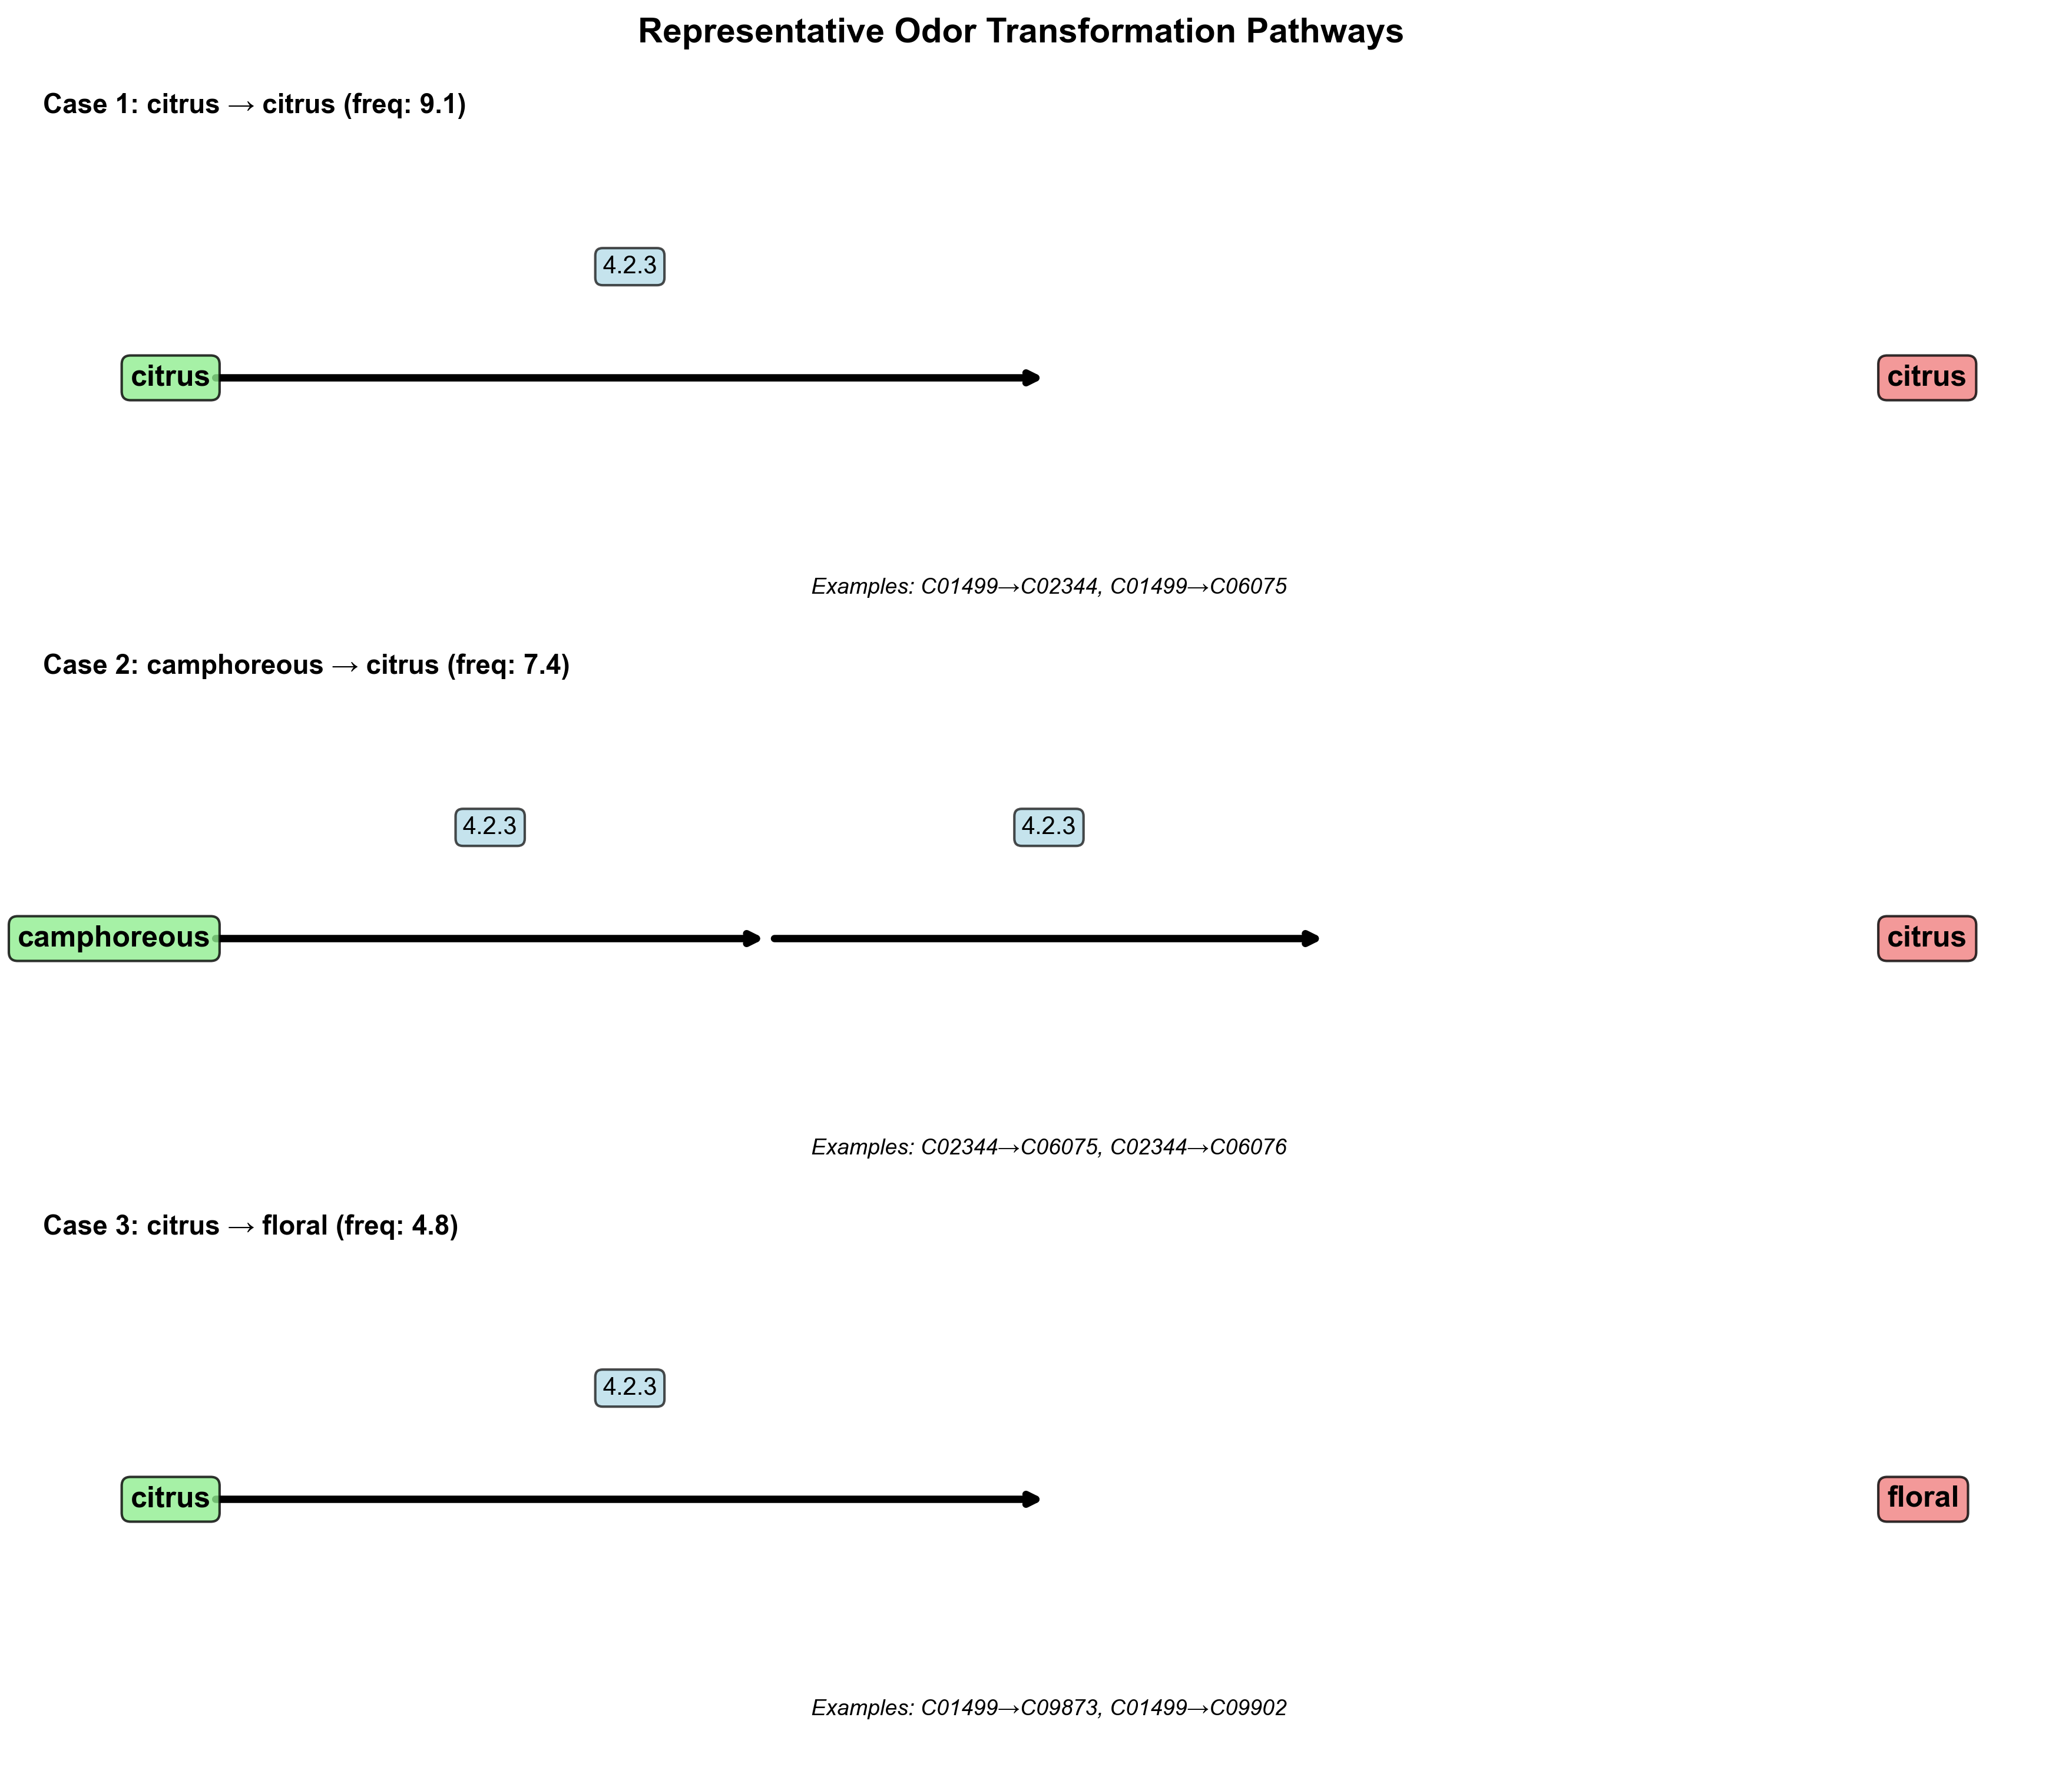
\includegraphics[width=0.95\linewidth]{09_case_studies.png}
\caption{Representative odor transformation pathways highlighting EC 4.2.3.}
\label{fig:case}
\end{figure}

\noindent\textbf{Reasoning examples and proof traces.}\label{sec:traces}

To demonstrate the inference engine in action, we present two complete reasoning examples that illustrate forward deduction with negation and consistency checking, respectively.

\noindent\textbf{Example 1: Forward reasoning with exclusion}

\noindent\textbf{Query:} \texttt{from(citrus), via([4.2.3]) $\rightarrow$ ?T}

\medskip\noindent The engine proceeds in three stages. First, an exclusion pass eliminates impossible targets: \texttt{excluded(citrus, `4.2.3', cheesy)} $\leftarrow$ Rule \#1042 (0.97), \texttt{excluded(citrus, `4.2.3', fishy)} $\leftarrow$ Rule \#1089 (0.95), and \texttt{excluded(citrus, `4.2.3', sulfurous)} $\leftarrow$ Rule \#1156 (0.93). Second, sufficient-condition rules predict reachable targets: \texttt{sufficient([4.2.3], fresh)} $\leftarrow$ Rule \#87 (0.89) and \texttt{sufficient([4.2.3], floral)} $\leftarrow$ Rule \#91 (0.85). Third, conditional-necessary rules add must-via constraints: \texttt{must\_via(citrus, citrus, `4.2.3')} $\leftarrow$ Rule \#4521 (0.92).

\noindent\textbf{Answer:} Top targets = \{fresh, floral, herbal, citrus\}. Excluded targets with reasons: cheesy (exclusion \#1042), fishy (exclusion \#1089), sulfurous (exclusion \#1156). The proof trace reveals that the answer is dominated by exclusion rules (negation reasoning) and supported by sufficient rules (generative prediction).

\noindent\textbf{Example 2: Consistency checking}

\noindent\textbf{Query:} Is the enzyme set $\{$EC~6.2.1, EC~4.2.3$\}$ consistent for a single pathway?

\medskip\noindent The engine checks mutual-exclusion rules, for example \texttt{mutual\_exclusive(`6.2.1', `4.2.3')} $\leftarrow$ Rule \#8934 (0.88).

\noindent\textbf{Answer:} \emph{Contradiction detected.} EC~6.2.1 (acid--CoA ligases) and EC~4.2.3 (carbon--oxygen lyases) are mutually exclusive in observed odor pathways. The proof trace identifies Rule \#8934 as the source of conflict, pointing to a possible mechanistic explanation: CoA-activation (ligase) and cyclization (lyase) operate on incompatible substrate states within single-pathway contexts.

\medskip
These examples illustrate the three-layer capability of the system: \emph{retrieval} (matching applicable rules), \emph{inference} (chaining rules to derive positive and negative conclusions), and \emph{explanation} (providing a human-readable proof trace for each step).

%% ============================================================
\section{Discussion}\label{sec:discussion}
%% ============================================================

\subsection{Lyase-dominated navigation of odor space}

The dominance of lyases (EC~4.x, 47.9\%) in odor-relevant pathways contrasts sharply with primary metabolism, where oxidoreductases and transferases predominate. Lyases catalyze elimination reactions---cleaving C--C, C--O, or C--N bonds to form double bonds or cyclic structures---generating the structural diversity of volatile odorants. Terpene cyclases (EC~4.2.3) convert linear prenyl diphosphates into cyclic monoterpenes; decarboxylases (EC~4.1.1) generate amines and aldehydes. The hub status of EC~4.2.3 (mediating transitions between citrus, fresh, herbal, and floral) suggests that \emph{odor space may be navigated principally through cyclization and elimination chemistry}. This interpretation is consistent with the catalytic promiscuity of lyases, but remains a hypothesis to be tested experimentally.

\subsection{Cartesian odor space as a reasoning interface}

Traditional SOR models position molecules as points in an embedding space. Our Cartesian odor event $(S, \mathbf{E}, T)$ introduces a fundamentally different formal object---one that binds a \emph{perceptual transition} to its \emph{mechanistic step sequence}. This design choice has two consequences. First, EC sequences are treated as transformation steps that act on perceptual states rather than as dimensions in a feature vector, mirroring how metabolism actually works: enzymes \emph{change} molecules, they do not \emph{describe} them. Second, by encoding events as typed predicates over odors and enzyme steps, the representation natively supports deduction (Q1), abduction (Q2), and contradiction detection (Q3) with proof traces; no post-hoc interpretation layer is needed because the representation itself is the language of inference.

This design provides a \emph{cognitive-level reasoning interface}: the $(S, \mathbf{E}, T)$ vocabulary aligns with how odors are described and manipulated in human knowledge (``citrus becomes floral through terpene cyclases''), making proof traces legible to domain experts without requiring machine-learning literacy. We do not claim to model neural circuits; we propose a reasoning interface aligned with the categorical and relational structure of human olfactory reports.

\subsection{Operator order and boundary constraints}

One of the most consequential observations is that odor transformations behave like an \emph{enzyme-sequence grammar}. Because rules are extracted over sequences of EC steps, order matters: the same enzymes can imply different odor transitions when applied in different sequences, demonstrating non-commutativity at the level of perceptual change. In parallel, exclusion and mutual-exclusion rules impose hard boundaries, indicating that certain odor targets are structurally or mechanistically inaccessible under specific steps or step pairs. These two properties---directionality and boundary constraints---are precisely what a purely structural embedding cannot represent. They motivate treating odor space as a rule-governed process rather than a static map, and they provide testable hypotheses about when and why an odor transition should fail.

Quantitatively, the boundary signal is strong: 8,072 exclusion rules have confidence 1.0, and 351 mutual-exclusion rules exceed 0.9 confidence. Directionality is not rare but systematic: among 733 conditional-necessary source$\rightarrow$target pairs, 566 are asymmetric. Non-commutativity is visible even in minimal two-step sequences; for example, \texttt{[1.8.1 -> 1.14.13]} yields sulfurous$\rightarrow$mint/cooling/camphoreous, whereas the reverse order \texttt{[1.14.13 -> 1.8.1]} yields phenolic$\rightarrow$burnt/sulfurous. These patterns are precisely the sort of boundary conditions and sequence rules that a static embedding omits but a mechanistic rulebook can state and test.

\subsection{From descriptive rules to auditable reasoning}

The shift from a static rule table to an executable inference engine represents a qualitative upgrade in the system's epistemic status. Static rules say ``\emph{this pattern exists}''; an inference engine says ``\emph{given these premises, this conclusion follows, and here is why}.'' Three properties distinguish the upgrade: falsifiability (predictions are backed by explicit enzymatic premises that can be tested and revised), compositionality (rules can be chained so exclusions, sufficient conditions, and necessities interact in a structured way), and auditability (proof traces explain \emph{why} a target odor is predicted or excluded rather than relying on an opaque score).

\subsection{Comparison with existing approaches}

Our approach complements rather than replaces structure-based odor models. The Principal Odor Map \citep{Lee2023} answers ``what does this novel molecule smell like?''; our framework answers ``\emph{how can that smell change, and why?}''. Multitask deep models \citep{Song2025} predict multiple odor labels from molecular graphs; our rules predict which transformations between labels are biochemically permitted, forbidden, or required. The relationship is analogous to the distinction between a map (POM) and a set of navigation rules (our rulebook): both are useful, and together they provide a more complete picture of olfactory space.

\subsection{External validation roadmap}

We outline three complementary validation approaches, ordered by effort. First, KEGG pathway cross-reference (implemented) traces high-confidence rules back to pathway IDs and documents the specific branch (e.g., citrus$\rightarrow$floral via \texttt{[4.2.3]} aligning with monoterpenoid biosynthesis and EC~4.2.3.25). Second, MetaCyc/BioCyc pathway matching would query EC sequences against curated pathway databases to assign biological-process names (e.g., fruit-ripening aroma formation, wine fermentation off-flavor production) to abstract rule patterns. Third, targeted literature validation would anchor rule-to-pathway matches in canonical food chemistry and plant biology sources (e.g., Ehrlich pathway in fermentation \citep{Hazelwood2008}; monoterpenoid biosynthesis in plants \citep{Tholl2015}), strengthening reviewer-facing evidence.

\subsection{Falsifiable hypotheses enabled by enzymatic rules}\label{sec:hypotheses}

A key advantage of executable rules over statistical associations is the ability to generate \emph{falsifiable} experimental predictions. We highlight three hypothesis families. The lyase-inhibition hypothesis states that if the conditional-necessary rule \texttt{from(citrus) $\wedge$ to(floral) $\rightarrow$ must\_via(4.2.3)} holds mechanistically, then inhibiting or deleting EC~4.2.3 lyases in a terpene-producing organism (e.g., \emph{Citrus sinensis} peel tissue or an engineered \emph{Saccharomyces cerevisiae} strain) should reduce citrus-to-floral aroma transitions as measured by gas chromatography-olfactometry (GC-O). The mutual-exclusion hypothesis posits that the rule \texttt{via(6.2.1) $\wedge$ via(4.2.3) $\rightarrow$ $\bot$} reflects incompatibility between CoA-ligase activation and terpene cyclization within a single viable pathway; metabolic flux analysis could test whether forced co-expression disrupts product profiles. The exclusion-violation hypothesis uses rules such as \texttt{from(citrus) $\wedge$ via([4.2.3]) $\rightarrow$ $\neg$to(cheesy)} to predict biochemically inaccessible transitions; engineering a pathway that violates such an exclusion would either strengthen the rule (if the target odor still fails to emerge) or refine its scope (if it does).

These hypotheses are directly readable from proof traces, illustrating how the reasoning system bridges computational analysis and bench-level experimental design.

\subsection{Limitations and future work}

The framework has several limitations. It relies on KEGG annotations, which may be incomplete for secondary metabolites and organism-specific pathways; TGSC odor labels are binary categories that can mask intensity gradients and context-dependent perception; rule confidence is statistical, derived from the observed transformation dataset, so psychophysical experiments are needed to confirm perceptual plausibility; and the current inference engine performs exact symbolic matching, so probabilistic or fuzzy reasoning (e.g., probabilistic logic programming such as ProbLog) could handle uncertainty more gracefully. Future work will extend the framework to organism-specific metabolic models, incorporate quantitative odor intensity data, and validate key rule predictions through targeted GC-O experiments.

%% ============================================================
\section{Conclusion}\label{sec:conclusion}
%% ============================================================

We have presented a transformation-centric framework for olfactory perception that bridges three traditionally separate disciplines: metabolic biochemistry, sensory neuroscience, and symbolic reasoning.

The framework introduces \emph{Cartesian odor events} $(S, \mathbf{E}, T)$ as a mid-level formal object that binds perceptual states to their enzymatic generators, enabling the extraction of 11,560 first-order logic rules across six categories of constraint. These rules are not merely descriptive---they are compiled into a Prolog-style inference engine that supports forward deduction, backward abduction, and consistency checking, with every conclusion accompanied by an explicit proof trace.

Two principal findings emerge. First, the analyses suggest that odor transitions are often mediated by cyclization and elimination chemistry: lyases (EC~4.x) account for 47.9\% of pathway steps, with EC~4.2.3 appearing as a recurrent hub enzyme mediating transitions between citrus, fresh, herbal, and floral categories. Second, the executable rulebook generates falsifiable biochemical hypotheses---linking enzymatic constraints to perceptual transitions in a form directly testable by GC-O and metabolic engineering experiments.

By shifting olfactory modeling from static molecule-to-odor mappings to \emph{queryable, mechanistically grounded, and logically auditable transformation rules}, this work offers a new paradigm for computational olfaction---one that explains not only what a molecule smells like, but how and why odors transform. The most disruptive implication is that odor space is structured by non-commutative enzyme sequences and boundary rules, not solely by static molecular structure.

All data, rules, interactive reasoning tools, and proof-trace demonstrations are publicly available.

% Author contributions
\printcredits

%% Bibliography
\bibliographystyle{cas-model2-names}
\bibliography{odor-refs}

\end{document}
